\documentclass[10pt,a4paper]{paper}
\usepackage[latin1]{inputenc}
\usepackage{amsmath}
\usepackage{amsfonts}
\usepackage{amssymb}
\usepackage{graphicx}
\usepackage{fancyvrb}
\usepackage[a4paper, total={7in, 8in}]{geometry}
<<<<<<< HEAD
\title{Guide into the WIOD R-package}
=======
\title{Introduction WIOD R package}
>>>>>>> f735e5d859ba5ae3846817921bc49efc9098d176
\author{Sybren Deuzeman}

\begin{document}
	\maketitle
	
	\section{Introduction}
	
<<<<<<< HEAD
	\section{Installing the WIOD R-package}
	
	\section{Load International Input Output Tables}
	
	The WIOD R-package comes with an easy way to easily import international input-output tables into our R environment. The data can be loaded in such a way that the different versions of international input-output tables can be used right away without the need to get the data into a workable format yourself. The data is, however, not delivered with the package as this would mean that the package becomes very large. Instead, the data is stored separately on the internet and can be downloaded with some pre-build functions. 
	
	There are two ways to use the WIOD R-package. The first is to download the data from the internet at use and the other is to create and use a local copy. Creating a local copy is advisable, since the data-files are relatively large. Since loading from the internet is the easiest to explain, we start with that. After that, we explain how to make a local copy and use that in a way very similar to loading from the internet.
	
	\subsection{Load from the Internet}
	
	In this section, we explain how to load the data using the internet and how the data itself is formatted. We start by downloading a international input-output table for a single year and version. Using this, we will explain the contents of an international. Next, we will explain how to load in a whole database of international input-output tables that is better suited for time-series analysis.
	
	\subsubsection{Load a Single IOT}
	\label{subsec:loadsingleiot}
	To load a single IOT, we can use the following function call \texttt{iot <- load\_iot("<version>", year)}.  For example, we can load international input-output table for 2000 from the World Input Output Database (WIOD) 2016 edition international input-output table using
	\begin{Verbatim}
	iot <- load_iot("WIOD2016", 2000)
	\end{Verbatim}
	
	This will load a large list that called \texttt{iot}. This list is the basic building block of the package as the build-up of these lists are the same for all different versions.
	
	The content of this list is:
	\begin{itemize}
		\item \texttt{I}: a matrix with the intermediate inputs use in one industry from another industry.
		\item \texttt{FD}: a matrix with different the final demand uses of the products of a sector. 
		\item \texttt{S}: a vector with the gross output of the sectors.
		\item \texttt{VA}: the value added of the sectors.
	\end{itemize}	
	
	After that follow some parameter that can be used by the program.
	\begin{itemize}
		\item \texttt{c}: number of countries in the input-output table
		\item \texttt{cf}: number of countries to which final demand goes.
		\item \texttt{n}: the number of industries. 
		\item \texttt{f}: the number of final demand categories. 
		\item \texttt{year}: the year for which the international input-output table is.
		\item \texttt{version}: the version of the international input-output table.
		\item \texttt{countries}: vector with the countries in the order in which they appear in the input-output table.
		\item \texttt{industries}: vector with the industries in the order in which they appear in the input-output table.
=======
	\section{Load International Input Output Tables}
	
	To be able to work with international input-output tables, we first need to load them into our program. There are two ways to do so: the first is to load the international input-output tables automatically into R. The other is to first make a local copy and then load it into R. The first method is useful if you either have a very strong internet connection or want to try the package. The second method is useful if you want to use the package intensively and do not want to download a lot of data every time you use the package. We first explain how to load international input-output tables from the internet. After that, we explain how to make a local copy and use that local copy.
	
	\subsection{Load from the Internet}
	
	To load data, one can use again two methods. The first one is loading a single international input output table. The second one is to load a set of input output tables into a list. The second method is most appropriate for executing the calculations on a set of input output tables, while the first one is most useful in creating your own personal methods with international input-output tables. We first explain how to load a single IOT and what the contents are, then we continue with loading the set of input-output tables. 
	
	\subsubsection{Single IOT}
	
	To load the World Input Output Database 2016 edition international input-output table for 2000, simply use
	\begin{verbatim}
		iot <- load_iot("WIOD2016", 2000)
	\end{verbatim}
	This will create the object iot, which is a large list. The list provided here is the basic building block of the package. These lists provide us with a way to make methods created with one version of the international input-output table compatible for use with other versions. The content of this list are shown in figure \ref{fig:contentiot} and is as follows:
	\begin{itemize}
		\item \texttt{I}: this is the block that describes the use of intermediate inputs from one industry being used by the other industry.
		\item \texttt{FD}: this contains data on the final demand used by other sectors. The $S$ block is the gross output of the industries.
		\item \texttt{VA}: is the value added by those industries. After that follow some parameter that can be used by the program.
		\item \texttt{c} is the number of countries in the input-output table
		\item \texttt{cf}: is number of countries for which we have data to which final demand goes.
		\item \texttt{n}: is the number of industries. 
		\item \texttt{f}: is the number of final demand categories. 
		\item \texttt{year}: is the year for which the international input-output table is.
		\item \texttt{version}: is the version of the international input-output table.
		\item \texttt{countries}: gives the countries in the order in which they appear in the input-output table.
		\item \texttt{industries}: gives the industries in the order in which they appear in the input-output table.
>>>>>>> f735e5d859ba5ae3846817921bc49efc9098d176
	\end{itemize}
	
	\begin{figure}[t]
	\centering
	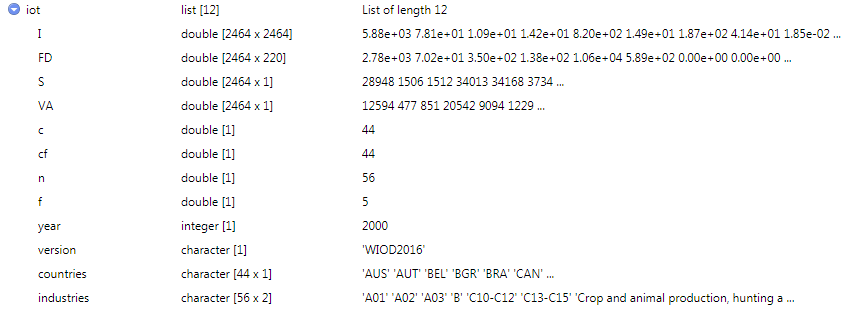
\includegraphics[width=\linewidth]{content_iot}
	\caption{The content of a Input-Output Table after loading it}
	\label{fig:contentiot}
	\end{figure}

<<<<<<< HEAD
	
	\subsubsection{List of IOTs}
	To obtain time-series, it is useful to load lists of IOTs instead of working with different single IOTs. The package comes with a function that can load such a list. To use the functions to export the results, one should also such lists instead of separate IOTs.
	
	One can load such a list of IOTs via the following command \texttt{iots <- load\_iots("<version>")}. To load the whole WIOD 2016 database at once, one can use the following code:
	\begin{Verbatim}
	WIOD2016 <- load_iots("WIOD2016").
	\end{Verbatim}
	Sometimes you would only want to load the data for a few years. We can do so by adding a vector with the years you want. To download the data of the WIOD 2016 database from 2005 to 2010 only, the following can be used:
	\begin{Verbatim}
	WIOD2016_0510 <- load_iots("WIOD2016", 2005:2010)
	\end{Verbatim}
=======
	The main idea of the package are that multiple versions are available. At the moment, three versions of international input output tables are available: the World Input Output Database (WIOD) from 2013 and 2016 and the Inter-Country Input-Output Tables (ICIOT) from 2018 of the OECD. To access other versions or other years, for example the Inter-Country Input-Output Tables of the OECD for 2005, simply use	
	\begin{verbatim}
		iot_iciot <- load_iot("ICIOT", 2005)
	\end{verbatim}
	
	\subsubsection{List of IOTs}
	Especially for calculation purposes, loading in a list of international input-output tables is advisable. The package comes with some functions that automatically executes a function for a single IOT over all the IOTs in such a list. Also, the functions to extract the calculated data from the input-output tables uses these lists. To load in the complete set of international input-output tables from the 2016 edition into such a list, simply use:
	\begin{verbatim}
		WIOD2016 <- load_iots("WIOD2016").
	\end{verbatim}
	If you want to only load the international input-output tables for some specific years, say from 2005 to 2010, use
	\begin{verbatim}
		WIOD2016_0510 <- load_iots("WIOD2016", 2005:2010)
	\end{verbatim}
>>>>>>> f735e5d859ba5ae3846817921bc49efc9098d176
	
	\subsection{Make a Local Copy}
	
	\subsection{Load Extra Data}
<<<<<<< HEAD
	In some cases, supplemental data needs to be downloaded. For example, the WIOD project database also consists of the Socio-Economic Accounts. This data can be added to the list via one of two functions \texttt{load\_extra\_iot} or \texttt{load\_extra\_iots}. To load the Socio-Economic Accounts (SEA) to the already loaded \texttt{iot}, you can use:
	\begin{Verbatim}
	iot <- load_extra_iot(iot, "SEA")
	\end{Verbatim} 
	To load the Socio-Economic Accounts to a list of IOTs, i.e. to the already loaded \texttt{WIOD2016}, you can use:
	\begin{Verbatim}
	WIOD2016 <- load_extra_iots(WIOD2016, "SEA")
	\end{Verbatim}
	
	
	\section{Use International Input Output Tables}
	We want to use International Input-Output Tables to generate new measures. For this, one can either build an own function as described in \ref{sec:ownfunction} or use one of the build-in functions. The functions are build to work with a single international input-output table. However, with the function \texttt{on\_iots} one can also use these functions on list of international input-output tables.
	
	\subsection{Use of package with single IOT}
	Here, we describe how to use a function and how these functions will behave in general. To do so, we consider the build-in function gii. This function  calculates the global import intensity of a specific sector as in [[CITATION]]. We will use function with \texttt{iot}, which we already downloaded:
	\begin{Verbatim}
	iot <- gii(iot)
	\end{Verbatim}
	We store the output of this function to the same list that we also used as argument for the function. We could have stored it as well into another list, which will then be a copy of the old list with new results added.
	
=======
	In some cases, extra data needs to be downloaded. For example, the WIOD project has also Socio-Economic Accounts. This data can be quite easily added to our list via either the \texttt{load\_extra\_iot} or \texttt{load\_extra\_iots} command. To load the Socio-Economic Accounts (SEA), one simply uses the following code for an already loaded iot:
	\begin{verbatim}
		iot <- load_extra_iot(iot, "SEA")
	\end{verbatim}
	This will add another list to the list with all data from the Socio-Economic Account. 
	To load the Socio-Economic Accounts to a list of IOTs, simply use
	\begin{verbatim}
		WIOD2016 <- load_extra_iots(WIOD2016, "SEA")
	\end{verbatim}
	
	
	\section{Use International Input Output Tables}
	To use the loaded Input-Output Tables to generate new measures, one can use some build-in functions on both a single IOT and on a list of multiple IOTs. We start again with the case of a single IOT to show what the package does in these cases. We first explain how to use the package with a single IOT and then with a list of multiple IOTs.
	
	\subsection{Use of package with single IOT}
	We use the build-in function GII, which calculates the global import intensity as in [[CITATION]] on the already loaded international input-output table $iot$. The code for this is:
	\begin{verbatim}
		iot <- gii(iot)
	\end{verbatim}
	Note that the output of this function need to be stored again. As done here, it can be stored again in the same object that is used to calculate. It can be stored in a new list, which will be a copy of the old list with the new calculations added.
>>>>>>> f735e5d859ba5ae3846817921bc49efc9098d176
	\begin{figure}
	\centering
	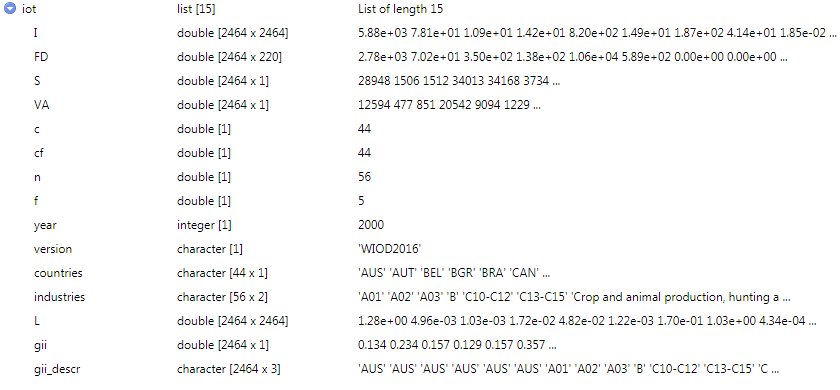
\includegraphics[width=1\linewidth]{content_iot_function}
	\caption{Content of \texttt{iot} after the command}
	\label{fig:contentiotfunction}
	\end{figure}

<<<<<<< HEAD
	In figure \ref{fig:contentiotfunction}, we show the contents of \texttt{iot} after using the function \texttt{gii}. Most part is as discussed in section \ref{subsec:loadsingleiot}. Three elements are added. The first is \texttt{L}, which is the Leontief inverse. As calculating the Leontief inverse is computationally intensive, we store the Leontief inverse for later use. Second, the element \texttt{gii} is added. In \texttt{gii}, the results of our calculations are stored. Third \texttt{gii\_descr} is added. In \texttt{gii\_descr}, we store the description of the data that can be used by our export functions.
	
	The function \texttt{gii} also has two other arguments, namely \texttt{regions} and \texttt{industries}. These arguments add region and industry categories to \texttt{gii\_descr}. To get a region categorization, one can use the function \texttt{countrycat}. As an example, we add a NAFTA and BeNeLux categorization:
	\begin{Verbatim}
	NAFTA <- c("USA", "MEX", "CAN")
	BENELUX <- c("BEL", "NLD", "LUX") 
	regions <- countrycat(list(NAFTA, BENELUX), iots)
	\end{Verbatim} 
	to create a region categorization. Finally, we use the \texttt{regions} argument as
	\begin{Verbatim}
	iot <- gii(iot, regions = regions)
	\end{Verbatim}
	to include the region categories to the data description.
	
	\subsection{Use of package with list of IOTs}
	If we use a list of international input-output tables, we can use the function \texttt{on\_iots}. The function \texttt{on\_iots} executes a function on all the input-output tables in the list. To use the function \texttt{gii} on all elements of the list \texttt{WIOD2016}, we can use
	\begin{Verbatim}
	WIOD2016 <- on_iots(gii, WIOD2016)
	\end{Verbatim}
	To add extra arguments, like te region categories as before, one can add extra arguments to the end of the function call, i.e.:
	\begin{Verbatim}
	WIOD2016 <- on_iots(gii, WIOD2016, regions = regions)
	\end{Verbatim}
	
	\section{Export Results}
	In the package, results are stored in a list of lists. Without some help, it is therefore not easy to extract the data for further analysis. To help us, the package includes two functions: \texttt{export\_dataframe} and \texttt{export\_csv}. The first function exports the data to an R dataframe. The second function exports the data into a CSV file, such that the results can be loaded into another program for further analysis.
	\subsection{Export to Dataframe}
	
	To extract the earlier calculated global import intensities from \texttt{WIOD2016} into a dataframe, we can use:
	\begin{Verbatim}
	gii_df <- export_dataframe("gii", WIOD2016)
	\end{Verbatim}
	This will generates a dataframe in ``wide'' format. Every year will have a separate column with its data. We can also export the data into ``long'' format. This does not store every year into a different variable, but gives the year for which it is in a separate column. This can be done via:
	\begin{Verbatim}
	gii_df_long <- export_dataframe("gii", WIOD2016, long = TRUE)
	\end{Verbatim}
	This function can be used to export the results of different functions. To add, for example, the total final demand for certain sectors, one can use
	\begin{Verbatim}
	WIOD2016 <- on_iots(fd_total, WIOD2016)
	gii_fvas_df <- export_dataframe(c("gii", "fd_total"), WIOD2016)
	\end{Verbatim}
		
	If \texttt{gii} and \texttt{fd\_total} would not have been of the same length, an error occurs. Further, the data description for \texttt{gii} will be used as this was the measure that is at the first position.
	
	\subsection{Export into a CSV file}
	The function \texttt{export\_csv} shares the same basic setup. The most simple way to use it is
	\begin{Verbatim}
	export_csv("gii", WIOD2016)
	\end{Verbatim}
	If one runs this code, a window will open to ask where to store the results. One can also add the file-path or filename directly via the directory argument:
	\begin{Verbatim}
	export_csv("gii", WIOD2016, directory = "C://Some/Dir/and/File.csv")
	\end{Verbatim}
	\section{Make Your Own Functions}
	\label{sec:ownfunction}
	The strength of this package is that you only need to write the function, while the rest of the package takes care of managing the data. The functions can be written for a single input-output table, while the rest of the package makes it easy to obtain results for a whole database of input-output tables.
	
	To aid in writing your own functions, we show the source code of the \texttt{gii} function:
	\begin{Verbatim}
	gii <- function(iot, regions = "None", industries = "None"){
		# Do necessary preliminary calculations
=======
	Figure \ref{fig:contentiotfunction} shows the contents of \texttt{iot} after we have used this function. Compared to before, three things. The first is \texttt{L}, which is the Leontief inverse. Finding the Leontief inverse involves inversing a, in this case, 2464 by 2464, matrix. That operation takes a considerable amount of time and we avoid that by storing the Leontief Inverse for later use. The second element that is added is \texttt{gii}, which stores the calculations. The third added element is \texttt{gii\_descr}, which describes for which country and sector that data is applicable. The third element will be used when we export the results.
	
	The function \texttt{gii} also allows for two other arguments, namely \texttt{regions} and \texttt{industries}. These arguments add region and industry categories to \texttt{gii\_descr}. To get an appropriate categorization, one can use the function \texttt{countrycat}. To add a NAFTA and BeNeLux categorization, one can use
	\begin{verbatim}
		NAFTA <- c("USA", "MEX", "CAN")
		BENELUX <- c("BEL", "NLD", "LUX") 
		regions <- countrycat(list(NAFTA, BENELUX), iots)
	\end{verbatim} 
	to create a region categorization. Finally, one can use
	\begin{verbatim}
		iot <- gii(iot, regions = regions)
	\end{verbatim}
	to include the region categories to the data description.
	
	\subsection{Use of package with set of IOTs}
	To execute $gii$ on the set of IOTs we have loaded before, we can use another function, namely \texttt{on\_iots}\footnote{\texttt{on\_iots} is basically the one-liner \texttt{iots <- lapply(iots, fun, ...)}.}. The function \texttt{on\_iots} executes a function on all the input-output tables in the list and the command to do so for the function \texttt{gii} on our list of IOTs \texttt{WIOD2016} is:
	\begin{verbatim}
		WIOD2016 <- on_iots(gii, WIOD2016)
	\end{verbatim}
	To add extra arguments, like te region categories, you can add these as extra arguments to \texttt{on\_iots}:
	\begin{verbatim}
	WIOD2016 <- on_iots(gii, WIOD2016, regions = regions)
	\end{verbatim}
	
	\section{Export Results}
	As explained before the results are stored in a list of lists. In this way, it is not easy to use our results elsewhere for further analysis. To extract the results from this list of lists, we can use two functions: \texttt{export\_dataframe} and \texttt{export\_csv}. The first function exports the data to an R dataframe. The second function exports the data into a CSV file.
	\subsection{Export into a Dataframe}
	
	To extract the global import intensities from \texttt{WIOD2016} into a dataframe, we can use:
	\begin{verbatim}
		gii_df <- export_dataframe("gii", WIOD2016)
	\end{verbatim}
	This generates a dataframe in ``wide'' format. For every year, there is a separate column. We can also export the data into ``long'' format, in which year is just another variable. To do so, we can use:
	\begin{verbatim}
		gii_df_long <- export_dataframe("gii", WIOD2016, long = TRUE)
	\end{verbatim}
	To add, for example, the total final demand for certain sectors, one can do so as well
	\begin{verbatim}
		WIOD2016 <- on_iots(fd_total, WIOD2016)
		gii_fvas_df <- export_dataframe(c("gii", "fd_total"), WIOD2016)
	\end{verbatim}	
	An error will occur when the outputs for \texttt{gii} and \texttt{fd\_total} are not of the same length. In this case, these however are of the same length, so that is not a problem. Note further that the data description for \texttt{gii} will be used as it is the first in the list.
	
	\subsection{Export into a CSV file}
	The function \texttt{export\_csv} has the same basic setup, although it does not store a dataframe within R. The most simple way is
	\begin{verbatim}
		export_csv("gii", WIOD2016)
	\end{verbatim}
	If one runs this code, a prompt window will open to ask where to store the results. That information can also be added in the code using the directory argument like this:
	\begin{verbatim}
		export_csv("gii", WIOD2016, directory = "C://Some/Dir/and/File.csv")
	\end{verbatim}
	\section{Make Your Own Functions}
	The strength of this package is that you only need to write the function, while the rest of the package takes care of managing the data. The functions can be written such that they function with a single input-output table. Using this for all years and for other versions of international input-output tables is taken care of by the WIOD package.
	
	To aid in writing your own functions, we add among the simplest, but still complete functions in our package: the \texttt{gii} function
	\begin{Verbatim}
	gii <- function(iot, regions = "None", industries = "None"){
		# Obtain some necessary preliminary calculations
>>>>>>> f735e5d859ba5ae3846817921bc49efc9098d176
		A <- coefficient(iot)
		iot <- leontief(iot)
	
		# Get results
		temp = matrix(1, iot$c, iot$c) # Create a c x c matrix with ones
		for (i in 1:iot$c){
			temp[i,i]=0 # make the diagonal into 0's
		}
		S = kronecker(temp, matrix(1, iot$n, iot$n)) 
		result <- t(colSums(S * A) %*% iot$L) 
		
		# Store results to the list
		iot$gii <- result	
		iot$gii_descr <- countryindustry_descr(iot, regions, industries)
		
		# Return the list
		return(iot)
	}	
	\end{Verbatim}
<<<<<<< HEAD
	The code is split in four parts. We will discuss these parts shortly.
	
	\paragraph{Do necessary preliminary calculations} Here some necessary calculations are done. We need to find the so called coefficient matrix and the Leontief matrix to calculate the GII. We do not store the coefficient matrix, \texttt{A} in the IOT list, but we do so for the Leontief inverse \texttt{L}. We want to calculate the Leontief inverse only once as it is computationally heavy and therefore we store it for later use. Finding the coefficient matrix is not computationally heavy, so we can find it every time we need it.
	
	\paragraph{Get results} Here, we do some calculations to get the necessary results. One can use elements from the IOT list using \texttt{iot\$element}. Observe that we use \texttt{colSums()} to find the sum over all elements of the columns. In R, element-wise manipulation is generally much faster than matrix manipulations. One should thus avoid matrix manipulation. 
	
	\paragraph{Store results to the list}
	The results are stored to the list of the input-output table via  \texttt{iot\$gii <- result}. Next, we add a description via another function \texttt{iot\$gii\_descr <- countryindustry\_descr(iot, regions, industries)}. 
	
	\paragraph{Return the list} The list \texttt{iot} that contains now, next to the original content, the Leontief inverse, the GII calculations and its accompanying data description is returned as the result of the function call.
=======
	First, we do some necessary calculations: namely the coefficient matrix \texttt{A} and the Leontief matrix \texttt{L}. Observe that we do not store the coefficient matrix into the input-output table, but we do store the Leontief matrix. Calculating the coefficient matrix is fast, while it is a large matrix to store. The Leontief matrix is as large to store, but calculating it takes a considerable amount of time.
	
	Next, we do some calculations to get the necessary results. Observe that we use \texttt{colSums()}, which gives the sum of all columns. In R, most matrix manipulations are not very efficient, while element-wise manipulation is much faster. In contrast with MatLab, it is therefore advisable to avoid the use of matrix manipulation as much as possible. Finally, the results are stored using \texttt{iot\$gii <- result}. We add a description via \texttt{iot\$gii\_descr <- countryindustry\_descr(iot, regions, industries)}. This list is then being returned from the function.
>>>>>>> f735e5d859ba5ae3846817921bc49efc9098d176
	\end{document}